\documentclass[12pt]{article}
\usepackage{url,amsmath,setspace,amssymb}
\usepackage{listings}

\usepackage{tcolorbox}
\usepackage{tikz}
\usepackage{xcolor}

\usepackage{color}

\usepackage{caption}
\usepackage{cite}

\usepackage[outputdir=build]{minted}
\usepackage{graphicx}
\graphicspath{ {./img} }

%**********************************************
%* Leave the page configuration as is
\setlength{\oddsidemargin}{.25in}
\setlength{\evensidemargin}{.25in}
\setlength{\textwidth}{6.25in}
\setlength{\topmargin}{-0.4in}
\setlength{\textheight}{8.5in}

\newcommand{\heading}[5]{
    \renewcommand{\thepage}{#1-\arabic{page}}
    \noindent
    \begin{center}
        \framebox[\textwidth]{
            \begin{minipage}{0.9\textwidth}
                \onehalfspacing
                {\textbf{\hfill} 650.045 -- \unitname}  #2

                    {\centering \Large #5

                }\medskip
                {#3 \hfill #4}
            \end{minipage}
        }
    \end{center}
}

%**********************************************


%**********************************************
%* Some more or less useful stuff

\lstnewenvironment{myalgorithm}[1][] %defines the algorithm listing environment
{
% \captionsetup{labelformat=algocaption,labelsep=colon}
    \lstset{ %this is the stype
        mathescape=true,
        frame=none,
        numbers=none,
        basicstyle=\normalsize,
        keywordstyle=\color{black}\bfseries\em,
        keywords={,input, output, return, datatype, function, in, if, else, foreach, while, begin, end, },
        numbers=left,
        xleftmargin=.04\textwidth,
        #1 % this is to add specific settings to an usage of this environment (for instance, the caption and referable label)
    }
}
{}



\newcommand{\unitname}{Advanced Topics in A.I. 2}
\newtcolorbox{alert}[1]{
    colback=red!5!white, colframe=red!75!white,fonttitle=\bfseries, title = #1}

\newtcolorbox{commentbox}[1]{
    colback=black!5!white, colframe=black!75!white,fonttitle=\bfseries, title = #1}
%**********************************************


%**********************************************
%* Please replace this with your name
\newcommand{\studentname}{Francesco Bombassei De Bona - 12138677}
%**********************************************
\newcommand{\handout}[3]{\heading{#1}{#2}{\studentname}{}{Mini-project: #3}}

%**********************************************
%* The document starts here
\begin{document}
    \handout{4}{Winter Term, 2022/23}{Reverse planning}


    \section{Introduction}\label{sec:intro}
    As mini-project I choose the proposed task A\@.
    The goal of this task is to implement a STRIPS planning domain where there is at least one action that is uniformly reversible.
    I implemented a domain both in PDDL and in K\@.


    \section{Project structure}\label{sec:structure}
    The project is structured as follows:
    \begin{itemize}
        \item \textbf{report.pdf}: this report
        \item \textbf{pddl}: contains the encoding of the domain in PDD and an example problem
        \item \textbf{k}: contains the encoding of the domain in K, an example problem and the background information for the problem
        \item \textbf{img}: contains the images used in this report
    \end{itemize}


    \section{Domain}\label{sec:domain}
    As domain I've chosen to imagine a moving company that has to move furniture between various locations.
    The company has to perform some actions in order to be able to move the furniture.
    After performing such actions, the company can move the furniture from one location to another.
    I identified the following actions:
    \begin{itemize}
        \item \textbf{assemble}: assemble a piece of furniture
        \item \textbf{disassemble}: disassemble a piece of furniture
        \item \textbf{pack}: pack a piece of furniture
        \item \textbf{unpack}: unpack a piece of furniture
        \item \textbf{load}: load a piece of furniture into a truck
        \item \textbf{unload}: unload a piece of furniture from a truck
        \item \textbf{move}: move a piece of furniture from one location to another
    \end{itemize}
    The company has to perform the following actions in order to be able to move a piece of furniture from one location to another:
    \begin{enumerate}
        \item disassemble the piece of furniture
        \item pack the piece of furniture
        \item load the piece of furniture into a truck
        \item move the truck to the destination location
        \item unload the piece of furniture from the truck
        \item unpack the piece of furniture
        \item assemble the piece of furniture
    \end{enumerate}
    Accordingly to the previous actions and to the domain description, I've defined the following predicates:
    \begin{itemize}
        \item \textbf{assembled}: a piece of furniture is assembled
        \item \textbf{packed}: a piece of furniture is packed
        \item \textbf{loaded}: a piece of furniture is loaded into a truck
        \item \textbf{moved}: a piece of furniture is moved from one location to another
    \end{itemize}
    To keep the domain simple and focus more on the uniformly reversible actions, I've decided to assume that the company don't track the location of the trucks.

    In Figure~\ref{fig:domain} there is a graphical representation of the domain states and effects of actions.
    \begin{figure}[ht]
        \centering
        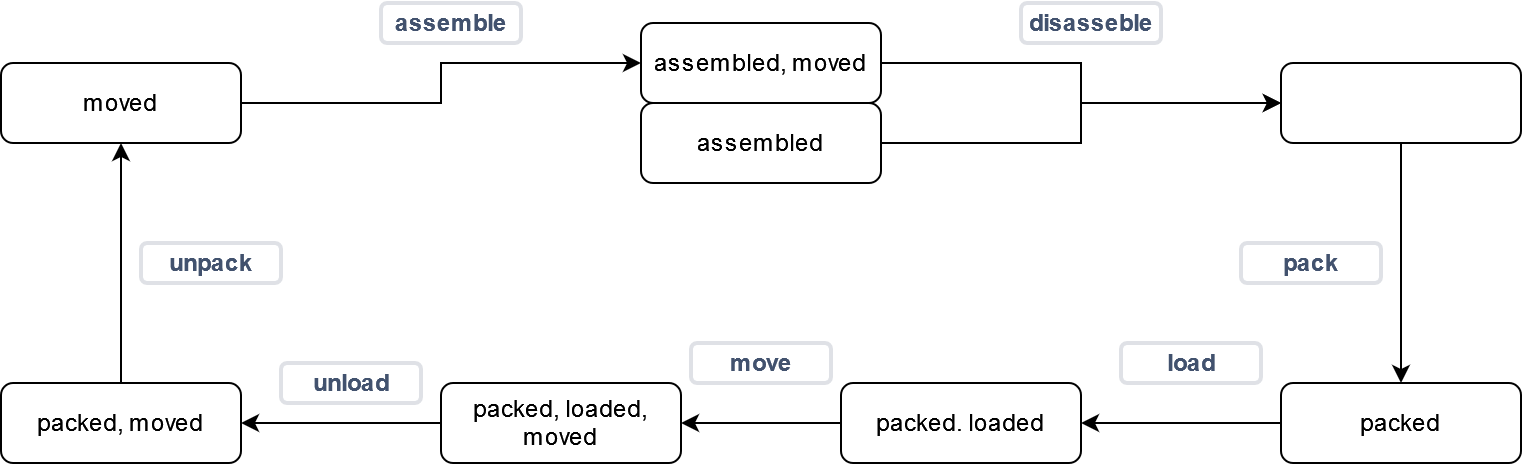
\includegraphics[width=\textwidth]{../img/diagram}
        \caption{Domain states and effects of actions}
        \label{fig:domain}
    \end{figure}

    \section{PDDL}\label{sec:pddl}

    \subsection{Domain description}\label{subsec:pddl-domain}
    The PDDL encoding of the domain is in the file \texttt{pddl/domain.pddl}.
    I defined two types of objects: \texttt{furniture} and \texttt{truck}.
    Each action has as parameters a piece of furniture and, additionally, the actions \texttt{load} and \texttt{unload} have as second parameter a truck.
    Every action has fixed preconditions over the four possible predicates, except for the action \texttt{disassemble} that is a valid action in any state were a piece of furniture was either moved or not.
    As for the effects, there are three couples of actions where each action of the couple is the reverse of the other, namely: \texttt{assemble} and \texttt{disassemble}, \texttt{pack} and \texttt{unpack} and \texttt{load} and \texttt{unload}.

    \subsection{Problem description}\label{subsec:pddl-problem}
    The PDDL encoding of the problem is in the file \texttt{pddl/problem.pddl}.
    The problem is defined as follows:
    \begin{itemize}
        \item \textbf{Initial state}: the initial state is defined as follows:
        \begin{itemize}
            \item \texttt{assembled} is true for the piece of furniture \texttt{couch} and \texttt{kitchen}
        \end{itemize}
        \item \textbf{Goal state}: the goal state is defined as follows:
        \begin{itemize}
            \item \texttt{assembled} is true for the piece of furniture \texttt{couch} and \texttt{kitchen}
            \item \texttt{moved} is true for the piece of furniture \texttt{couch} and \texttt{kitchen}
        \end{itemize}
    \end{itemize}
    The problem is solvable by the planner and the solution is the represented in Figure~\ref{fig:pddl-solution}.
    \begin{figure}[ht]
        \centering
        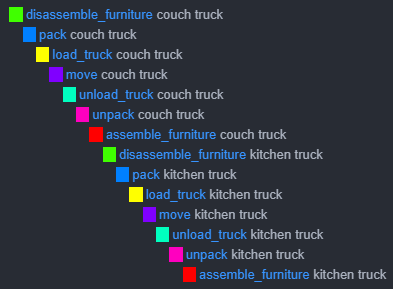
\includegraphics[width=\textwidth]{../img/pddl_problem_solution}
        \caption{Solution to the problem}
        \label{fig:pddl-solution}
    \end{figure}

    \subsection{Uniformly reversible actions}\label{subsec:pddl-reversible}
    Starting from the two previous files, I produced the translation of the domain and the problem in the \texttt{ASP} format.
    The shell command used to produce the translation is the following:
\begin{minted}[fontsize=\footnotesize]{shell}
plasp translate domain.pddl problem.pddl | cat - <(echo "\#show chosen/1.") > domain.lp
\end{minted}
    As for the previous command, to the original translation I added the directive \texttt{\#show chosen/1.} to show the chosen actions.
    Using the command \mintinline[breaklines, breakafter=_]{shell}{clingo domain.lp --const horizon=6 sequential-horizon.uurev.lp -n 0} I could find all the uniformly reversible actions.
    As expected, there are six actions that are uniformly reversible where only one plan reverse the initial state to the state previous to the chosen action.
    The uniformly reversible actions are the following:
    \begin{itemize}
        \item \texttt{assemble}
        \item \texttt{pack}
        \item \texttt{unpack}
        \item \texttt{load}
        \item \texttt{unload}
        \item \texttt{move}
    \end{itemize}
    In the Figure~\ref{fig:pddl-reversible} I show the six uniformly reversible actions and the plan that reverse the initial state to the state previous to the chosen actions.
    For simplicity, I've changed the background information of the problem to have only one piece of furniture and one truck.
    Changing the background information of the problem doesn't affect the uniformly reversible actions, that increase proportionally to the number of pieces of furniture and trucks.
    \begin{figure}[ht]
        \centering
        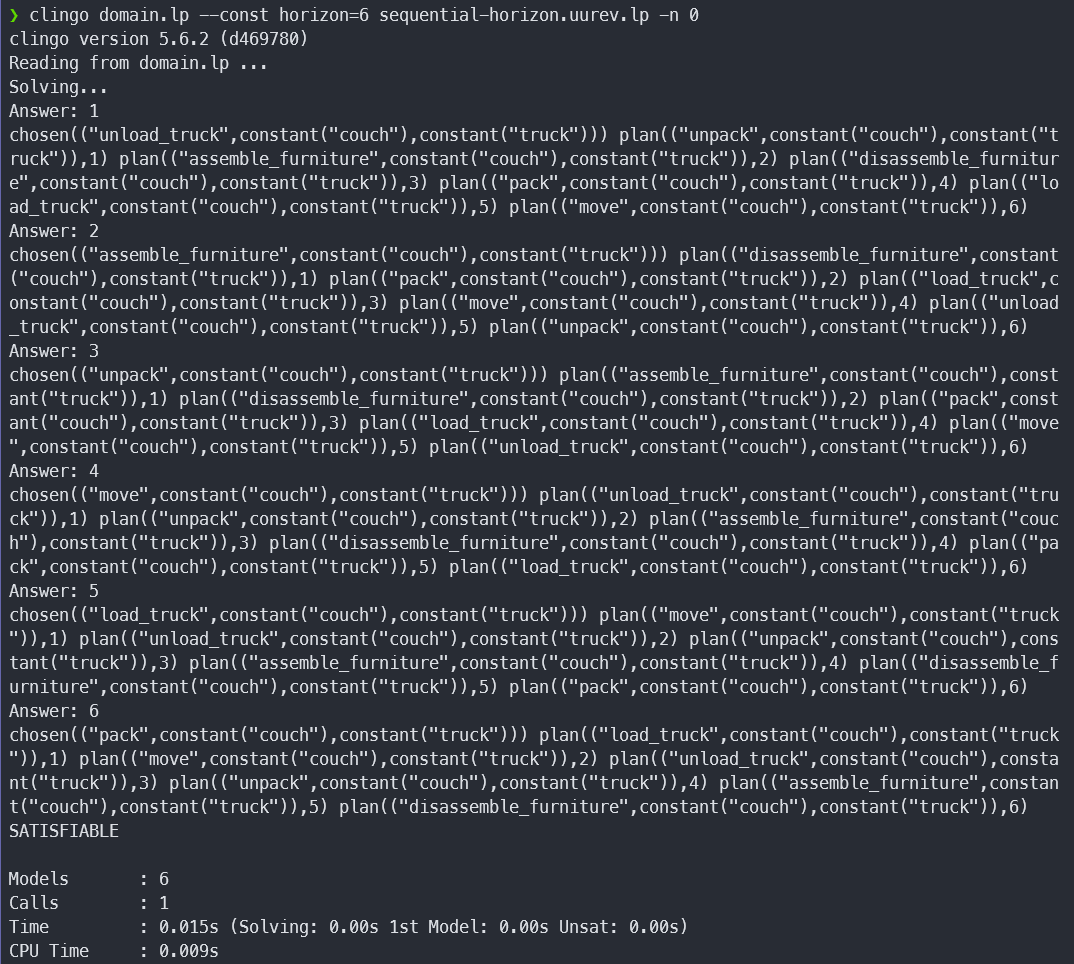
\includegraphics[width=\textwidth]{../img/unif_rev_actions}
        \caption{Uniformly reversible actions}
        \label{fig:pddl-reversible}
    \end{figure}
    The action \texttt{disassemble} is not uniformly reversible because there are two different initial states for the action, as shown in Figure~\ref{fig:domain}, and only one has a reverse plan that reverse the initial state to the state previous to the chosen action (the one where it holds that \texttt{\{assembled, moved\}} is true for the piece of furniture).

    \section{K}\label{sec:k}
    \subsection{Domain and problem description}\label{subsec:k-domain}
    The same domain and problem described in Section~\ref{sec:pddl} can be encoded in the \texttt{K} language.
    The \texttt{K} encoding of the domain is in the file \texttt{k/k\_domain.plan}.
    The \texttt{K} encoding of the problem is in the file \texttt{k/k\_problem.plan}.
    The \texttt{K} encoding of the domain is analogous to the one presented in the PDDL section.
    It was necessary to add the \texttt{inertial} property to all the fluents and to specify the \texttt{noConcurrency} option.
    Also a file containing the background information of the problem was necessary, just to specify the initial objects in the problem.

    Running the $\text{DLV}^k$ planner on the domain and the problem resulted in the same solution as the one found by the PDDL planner.
    This can be seen in Figure~\ref{fig:k-solution}.
    \begin{figure}[ht]
        \centering
        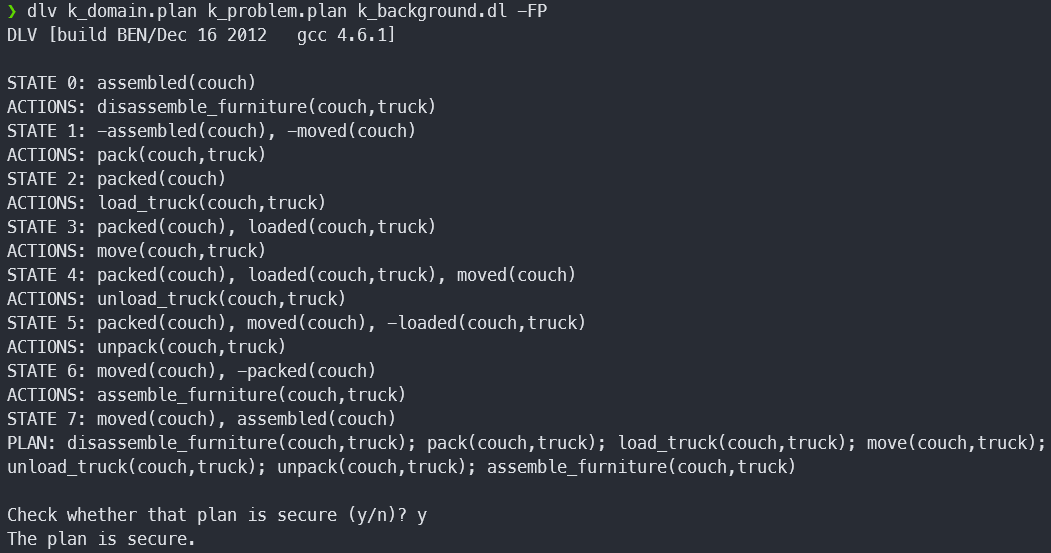
\includegraphics[width=\textwidth]{../img/k_problem_solution}
        \caption{Solution to the problem}
        \label{fig:k-solution}
    \end{figure}

    \subsection{Reverse plan}\label{subsec:k-reverse}
    I tried to use \texttt{revplan} software to find the reverse plan of the solution found by the $\text{DLV}^k$ planner but after running the command \mintinline[breaklines, breakafter=_]{shell}{java -cp plan-library-binary.jar planlibrary.ReverseDomain -x k_domain.plan k_background.dl cond.xml /usr/bin/dlv 15} for more than 24 hours, the software didn't find terminate at all (Figure~\ref{fig:k-reverse}).
    \begin{figure}[ht]
        \centering
        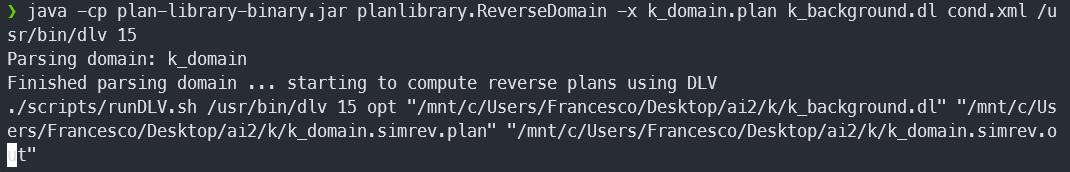
\includegraphics[width=\textwidth]{../img/k_reverse}
        \caption{Reverse plan}
        \label{fig:k-reverse}
    \end{figure}
    Even if the software didn't terminate, from the uniformly reversible actions retrieved in Section~\ref{subsec:pddl-reversible} and what shown in Figure~\ref{fig:domain}, I can state that the reverse plan for each combination of furniture and goal state corresponds to the plan to reverse each single uniformly reversible action.

    Only the cases of the goal states \texttt{\{assembled\}} and \texttt{\{assembled, moved\}} must be discussed.
    Regarding the second case, the reverse plan corresponds to the concatenation of the actions \texttt{\{disasseble, pack, load, move, unload, unpack, assemble\}}.
    The first case instead has no reverse plan because there is no actions sequence that can remove the single predicate \texttt{moved} from the state \texttt{\{assembled, moved\}}.
\end{document}